\documentclass[usenames,dvipsnames]{beamer}

\usepackage[utf8]{inputenc}
\usepackage{ngerman}
\usepackage{amsmath}
%\usepackage[T1]{fontenc}
\usepackage[compress]{beamerthemeBoadilla}
\usecolortheme{rose}
\usepackage{graphicx}
\usepackage{colortbl}
\usepackage{xcolor}

\definecolor{shadecolor}{gray}{.95}

\beamertemplatenavigationsymbolsempty

%Transparente Overlays:
%\setbeamercovered{transparent}

%Universitätssiegel:
%\pgfdeclareimage[height=0.7cm]{Siegel}{img/siegel.pdf}
%\logo{\pgfuseimage{Siegel}}

%%%%%%%%% FARBEN %%%%%%%%%%%

\definecolor{lightgray}{gray}{.92}
\definecolor{lightblue}{rgb}{0.8,0.85,1}
\definecolor{lightgreen}{rgb}{0.8,1,0.85}
\definecolor{lightred}{rgb}{1,0.75,0.7}
\definecolor{lightyellow}{rgb}{1,0.99,0.65}

%%Cellpadding
\setlength{\tabcolsep}{0.1cm}
\renewcommand{\arraystretch}{1.5}


\title{CEP am Beispiel von Esper}
\subtitle{\scriptsize Seminar - Event Driven Architectures}
\institute{}
\author{Martin Steinbach}
\date{Januar 2019}

\begin{document}


\part{Startfolie}
\begin{frame}
\titlepage
\end{frame}




\part{Vortrag}
%%%%%%%%%%%%%%%%%%%%%%%%%%%%%%%%%%%%%%%%%%%%%%%%%%%%%
\section{Grundlagen CEP}


\begin{frame}{\textbf{C}omplex \textbf{E}vent \textbf{P}rocessing}

\begin{exampleblock}{}
    \begin{itemize}
        \item  Analyse von unendlichen Ereignisströmen  
    \end{itemize}
\end{exampleblock}

\begin{center}
   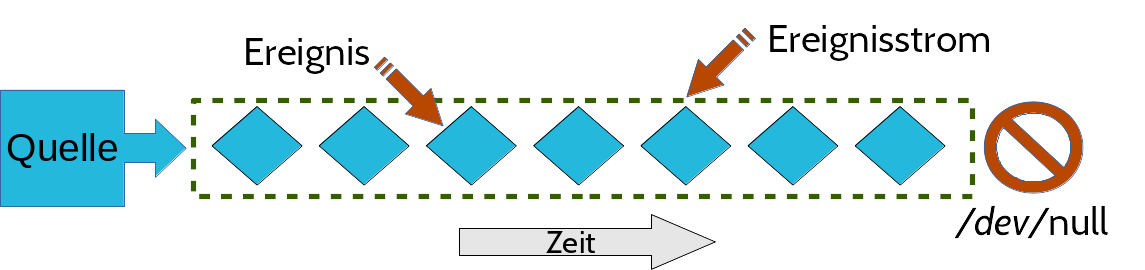
\includegraphics[scale=0.4]{img/01_cep}
\end{center}


\end{frame}

\begin{frame}{Komplexe Ereignisse}

\begin{exampleblock}{}
    \begin{itemize}
        \item Ereignismuster beschreiben Beziehungen zwischen Ereignissen
        \item Komplexe Ereignisse sind Abstraktionen von Ereignismengen
    \end{itemize}
\end{exampleblock}

\begin{center}
    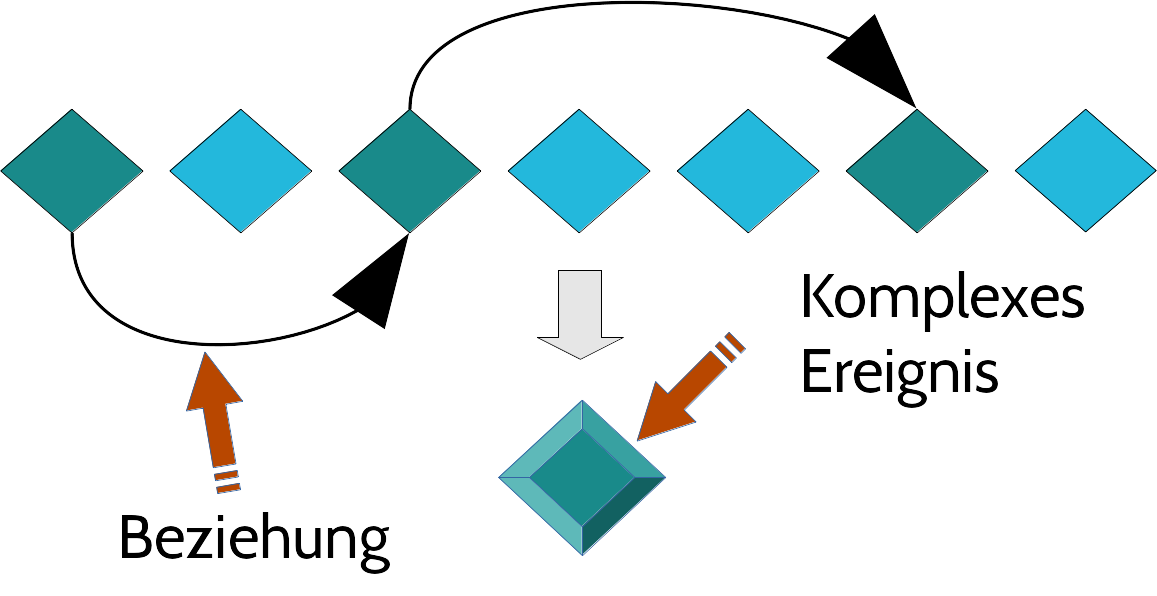
\includegraphics[scale=0.3]{img/02_cep}
\end{center}

\end{frame}



\begin{frame}{Ereignismuster}

\begin{exampleblock}{}
    \begin{center}
        \textbf{A} vor \textbf{C} vor \textbf{D}    
    \end{center}
\end{exampleblock}

\begin{center}
    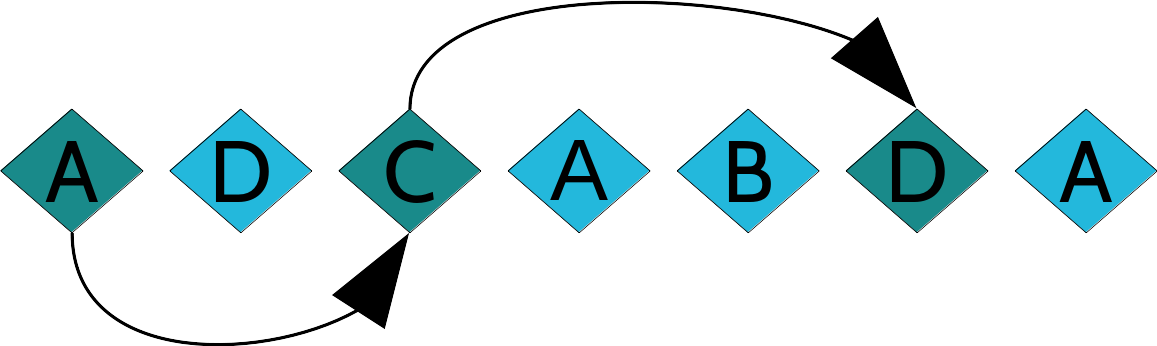
\includegraphics[scale=0.3]{img/03_cep}
\end{center}
\begin{exampleblock}{}
    \begin{center}
        \textbf{Ereignistypen}  
    \end{center}
\end{exampleblock}


\begin{center}
    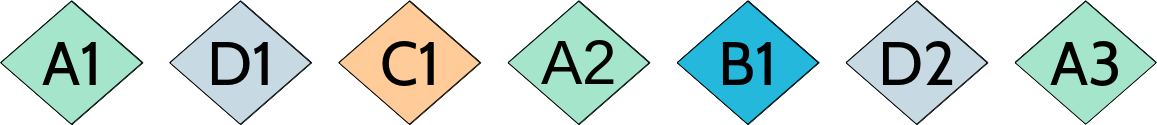
\includegraphics[scale=0.3]{img/04_cep}
\end{center}

\end{frame}

\begin{frame}{Ereignis in CEP}


\begin{columns}

\begin{column}{0.5\textwidth}
\begin{table}[ht]
    \centering{
        \renewcommand{\arraystretch}{1.1}
        \begin{tabular}{|l|c|}
            \hline
            \multicolumn{2}{|l|}{\cellcolor{shadecolor}\textbf{Metadaten}}\\
            \hline
            Ereignistyp\hspace{0.2cm} &   \texttt{Kursänderung}\\ 
            \hline
            Ereignisquelle\hspace{0.5cm} &   \texttt{Frankfurt}\\ 
            \hline 
            Zeitstempel &   \texttt{21:19:55}\\
            \hline
            ID          &   \texttt{98127634}\\  
            \hline
            \multicolumn{2}{|l|}{\cellcolor{shadecolor}\textbf{Kontextinformation}}\\     
            \hline
            \multicolumn{2}{|l|}{\texttt{Name: GCME AG}}\\
            \multicolumn{2}{|l|}{\texttt{Aktueller Kurs: 42.1}}\\
            \hline
        \end{tabular} 
    }
\end{table}
\end{column}
\begin{column}{0.4\textwidth}
    \begin{exampleblock}{}
        \begin{itemize}
            \item Aufbereitete Rohdaten
            \vspace{0.6 cm}
            \item Strukturiert
            \vspace{0.6 cm}
            \item Maschinenlesbar
            \vspace{0.6 cm}
            \item Atomar
        \end{itemize}
    \end{exampleblock}
\end{column}
\end{columns}
\end{frame}


%%%%%%%%%%%%%%%%%%% ESPER %%%%%%%%%%%%%%%%%%%%%%%%%%
\section{Esper}
\begin{frame}{}
\begin{center}
    \Large \textbf{ESPER I}
\end{center}

\vspace*{1cm}

\begin{tabular}{ll}
    Free Software (GPLv2) \hspace{3cm}   &\\
                            &CEP-Engine \\
    \hspace{2cm}\textbf{E}vent \textbf{P}rocessing \textbf{L}anguage & \\
                            &\hspace{2cm}\texttt{Java} und \texttt{C\#} \\ 
    \hspace{1cm}EPL $\rightarrow$ Bytecode&\\
        & SQL - \texttt{MATCH\_RECOGNIZE}\\
\end{tabular}
\end{frame}


\begin{frame}{ESPER II}
     \begin{center}
        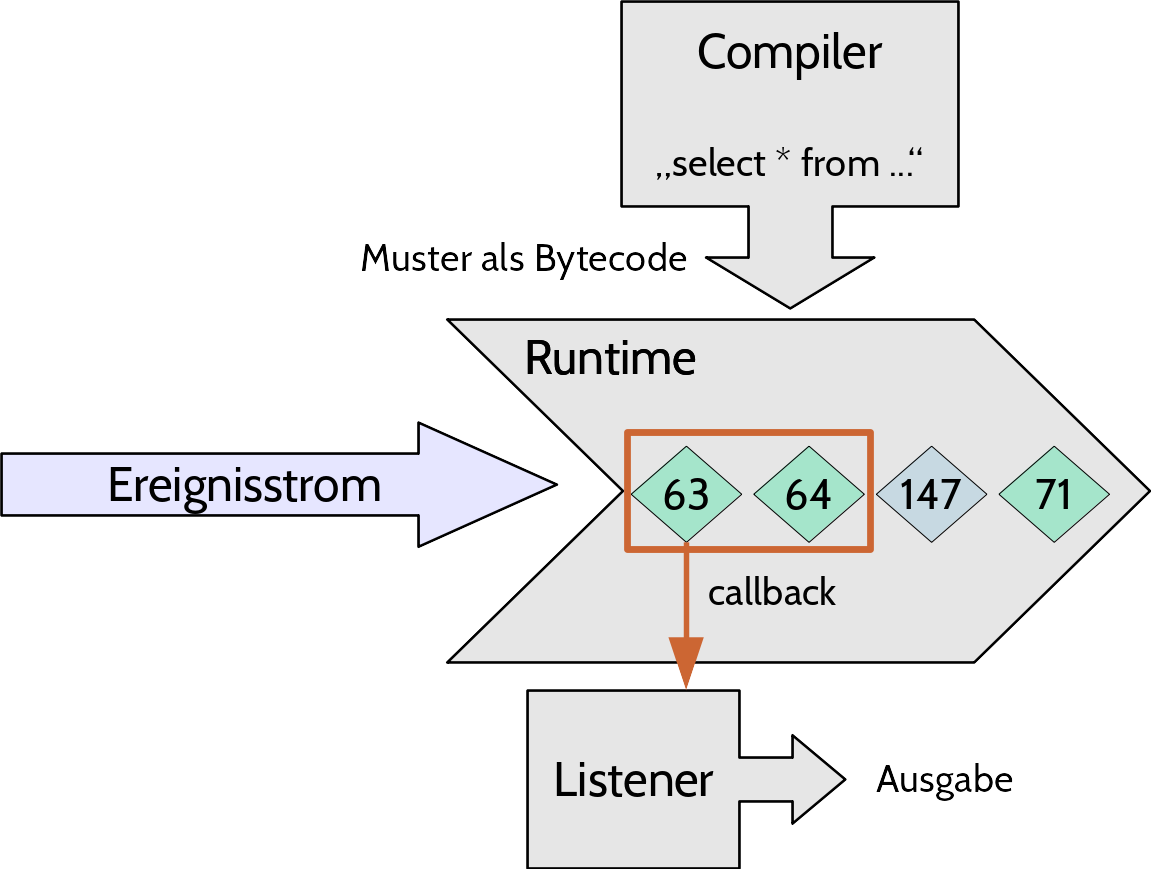
\includegraphics[scale=0.3]{img/esper}\hspace*{1cm}
    \end{center} 
\end{frame}


        





\begin{frame}{Musterdefinition - EPL/SQL}

\begin{exampleblock}{\textbf{E}vent \textbf{P}rocessing \textbf{L}anguage}
    \begin{itemize}
        \item Syntax ähnlich SQL
        \item Beschreibung durch Aussagenlogik + spezielle Operatoren
        \item Operiert auf unterschiedlichen Ereignistypen
    \end{itemize}

\end{exampleblock}

\begin{exampleblock}{SQL-Erweiterung: \texttt{MATCH\_RECOGNIZE}}
\begin{itemize}
    \item Einbettung in EPL-Anfrage
    \item Standardisiert in SQL:2016 (ISO/IEC 9075:2016)
    \item Beschreibung durch reguläre Ausdrücke
    \item Operiert auf einem Ereignistyp
\end{itemize}
\end{exampleblock}
   
\end{frame}

\begin{frame}{EPL-Operatoren}

\begin{block}{\centering wichtige Operatoren von EPL}
    \begin{tabbing}
        \texttt{A and B}:\hspace{3cm}  \=   A $\land$ B, Reihenfolge egal\\\\
        \texttt{A or B}: \>     A $\lor$ B, Reihenfolge egal\\\\
        \texttt{A -> B}: \>     Sequenz, B tritt zeitlich nach A ein\\\\
        \texttt{(A -> B) and not C}: \>     kein C vor A oder B\\\\
        \texttt{every A}: \>        detektiert alle A im Strom\\\\
        \texttt{[5] A}: \> Repeat, Detektion nach 5 A          
        
    \end{tabbing}
\end{block}


\end{frame}


\begin{frame}{Esper - Ereignistypen}
\begin{columns}   
    \begin{column}{0.5\textwidth}
        
        \begin{center}
            \hspace{1cm}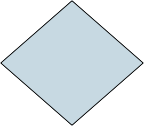
\includegraphics[scale=0.3]{img/ereignis_aa}
            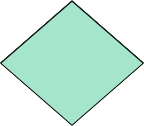
\includegraphics[scale=0.3]{img/ereignis_a}
        \end{center} 
        
    \end{column}
    
    \begin{column}{0.5\textwidth}
        \begin{center}
            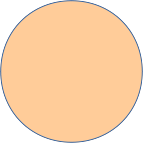
\includegraphics[scale=0.3]{img/ereignis_b}
        \end{center}  
        
    \end{column}
\end{columns}

\begin{tabbing}
    \textbf{Ereignistyp}:\hspace{0.2cm} \= StockTick \hspace{3cm} \= NewsTick\\
    \>\>\\
    \textbf{symbol:} \> 'IBM'/'SAP' \>'IBM'\\
    \textbf{price:} \> Integer \> -\\
    \textbf{message:} \> - \> 'good'/'bad'
\end{tabbing}

\begin{columns}   
    \begin{column}{0.5\textwidth}
        \begin{center}
            \hspace{1cm}
\includegraphics[scale=0.3]{img/ereignis_aa1}
            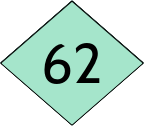
\includegraphics[scale=0.3]{img/ereignis_a1}
        \end{center} 
    \end{column} 
    \begin{column}{0.5\textwidth}
        \begin{center}
            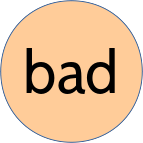
\includegraphics[scale=0.3]{img/ereignis_b1}
        \end{center}  
        
    \end{column}
\end{columns}
\end{frame}


\begin{frame}{EPL - einfache Anfragen}
    \begin{center}
        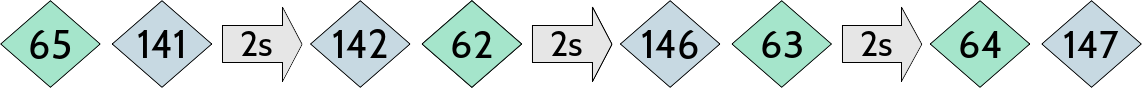
\includegraphics[scale=0.35]{img/stream-1}
    \end{center}    

\begin{exampleblock}{\centering EPL - einfache Anfragen}
    \begin{center}
         \texttt{\textcolor{red}{select} PARAMETER \textcolor{red}{from} SOURCE 
            \textcolor{red}{where} CONDITION;}
    \end{center}
\end{exampleblock}

\begin{exampleblock}{\centering Eine einfache Anfrage}
    \begin{center}
        \texttt{select * from StockTick where price > 100;}\\
        $=$\\
        \texttt{select * from StockTick\textcolor{red}{(}price > 100\textcolor{red}{)};}
    \end{center}
\end{exampleblock}

\begin{center}
    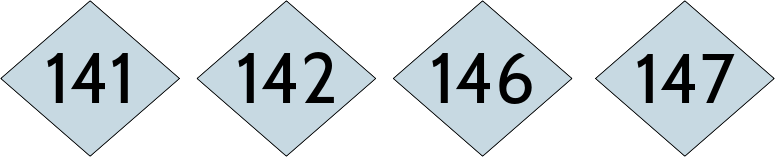
\includegraphics[scale=0.2]{img/solution-1}$\dots \infty$
\end{center}
\end{frame}





\begin{frame}{EPL - einfache Anfragen}
\begin{center}
    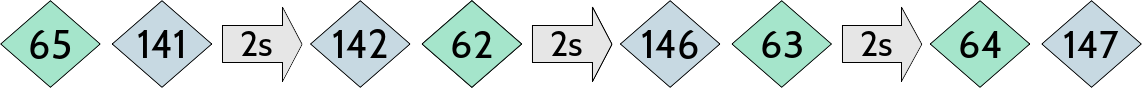
\includegraphics[scale=0.35]{img/stream-1}
\end{center}
\begin{exampleblock}{\centering Aggregation}
    \begin{center}
        \texttt{select avg(price) from StockTick(symbol='IBM')}
    \end{center}
\end{exampleblock}
\begin{center}
    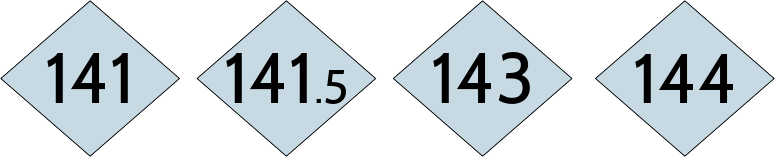
\includegraphics[scale=0.2]{img/solution-2}$\dots \infty$
\end{center}

\pause
\begin{alertblock}{}
    \begin{itemize}
        \item Operationen auf $\infty$-Datenstrom
        \item Anfragen würde ewig Ereignisse erstellen
    \end{itemize}
\end{alertblock}

\end{frame}

\begin{frame}{Fenster - einfache Zeitfenster}

\begin{exampleblock}{}
    \begin{center}
        \texttt{select  avg(price) from StockTick\textcolor{red}{.win:time(6 sec)} where 
        symbol='IBM'}
    \end{center}
\end{exampleblock}

\begin{center}
    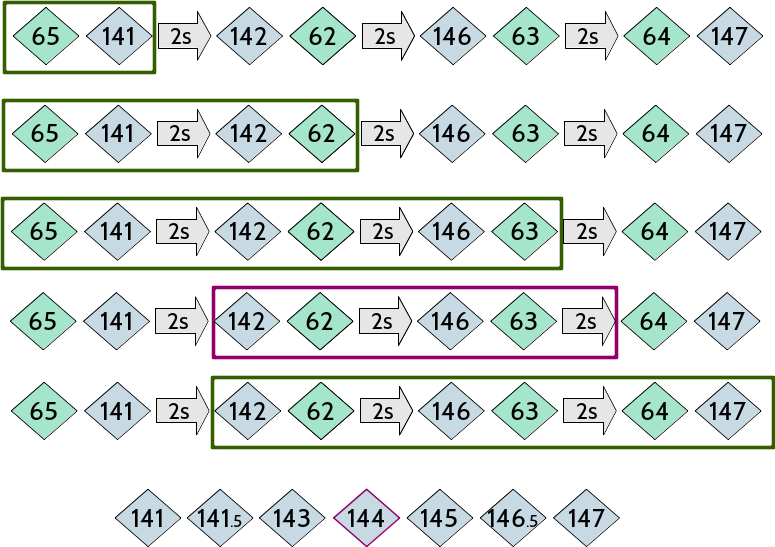
\includegraphics[scale=0.40]{img/solution-3}
\end{center}

\end{frame}

\begin{frame}{Fenster - \texttt{batch}-Zeitfenster}
\begin{exampleblock}{}
    \begin{center}
        \texttt{select  avg(price) from StockTick.win:time\textcolor{red}{\_batch}(6 sec) 
        where symbol='IBM'}
    \end{center}
\end{exampleblock}
\vspace{1cm}
\begin{center}
    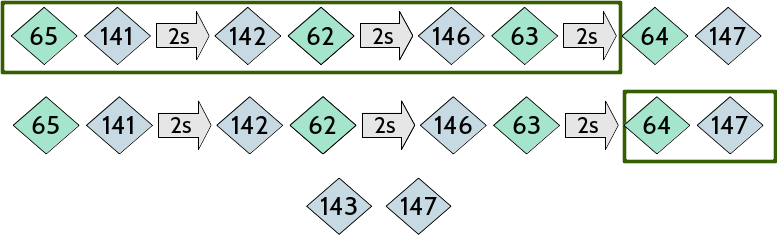
\includegraphics[scale=0.5]{img/solution-4}
\end{center}
\end{frame}
\begin{frame}{\texttt{Fenster - batch}-Längenfenster}
\begin{exampleblock}{}
    \begin{center}
        \texttt{select  avg(price) from 
        StockTick.win:\textcolor{red}{length\_batch}(4) where symbol='IBM'}
    \end{center}
\end{exampleblock}
\vspace{1cm}
\begin{center}
    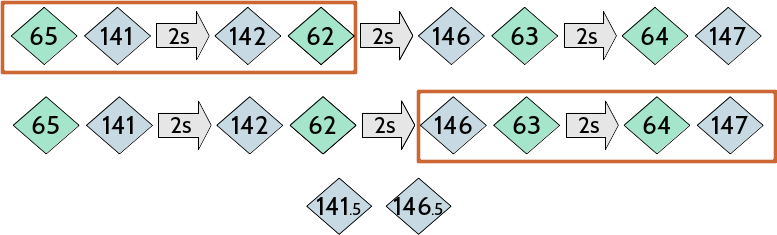
\includegraphics[scale=0.5]{img/solution-5}
\end{center}

\end{frame}

%EREIGNISTYPBASIERTE REGELN
\begin{frame}{Ereignistypbasierte Regeln}


\begin{block}{\centering \texttt{pattern[]}}
    \begin{itemize}
        \item Betrachtung unabhängig von Zeit und Länge
        \vspace{0.2cm}
        \item boolesche Ausdrücke + Sequenzoperator: $\rightarrow$
        \vspace{0.2cm}
        \item \texttt{pattern[A $\rightarrow$ B]}
        \begin{itemize}
            \item \texttt{A, B} sind Ereignistypen
            \item \texttt{a,b} deren Instanzen
            \item B tritt zeitlich nach A ein
            \item A ist Initiator, B ist Detektor 
        \end{itemize}
    \vspace{0.2cm}
        \item \texttt{every}-Operator (\textit{Event Consumption Modes})
    \end{itemize}
\end{block}

\end{frame}

\begin{frame}{Ereignistypbasierte Regeln}
\begin{center}
    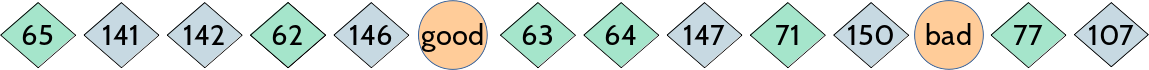
\includegraphics[scale=0.4]{img/stream-2}
\end{center}
\hspace{3cm}
\begin{exampleblock}{}
    \begin{center}
    \texttt{select \textcolor{red}{b} from 
    \textcolor{red}{pattern[a=StockTick(symbol='IBM') $\rightarrow$ 
    b=StockTick(symbol='SAP')]};}
\end{center}
\end{exampleblock}
\hspace{3cm}
\begin{center}
    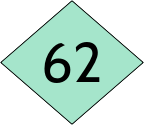
\includegraphics[scale=0.25]{img/solution-a}
\end{center}

%\begin{exampleblock}{}
%\begin{center}
%    \texttt{select b from pattern[a=StockTick(symbol='IBM') \textcolor{red}{and} 
%    b=StockTick(symbol='SAP')];}
%\end{center}
%\end{exampleblock}
%\begin{center}
%    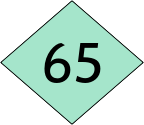
\includegraphics[scale=0.25]{img/solution-b}
%\end{center}
\end{frame}

\begin{frame}{Ereignistypbasierte Regeln - Consumption Modes I}
\begin{center}
    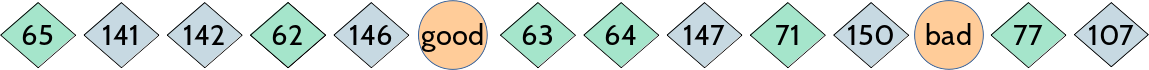
\includegraphics[scale=0.4]{img/stream-2}
\end{center}
\begin{exampleblock}{\textit{Unrestricted Consumption Mode:}}
    \begin{center}
        \texttt{pattern[ \textcolor{red}{every} A $\rightarrow$ \textcolor{red}{every} 
        B]}\\\vspace{0.3cm}
        \texttt{select a,b from pattern[\textcolor{red}{every} a=StockTick(symbol='IBM') 
        $\rightarrow$ 
            \textcolor{red}{every} b=StockTick(symbol='SAP')];}
        \end{center}
        \begin{itemize}
            \item Jeder Initiator konsumiert alle Detektoren
            \item sehr große Ergebnismenge
        \end{itemize}
    \end{exampleblock}

\begin{center}
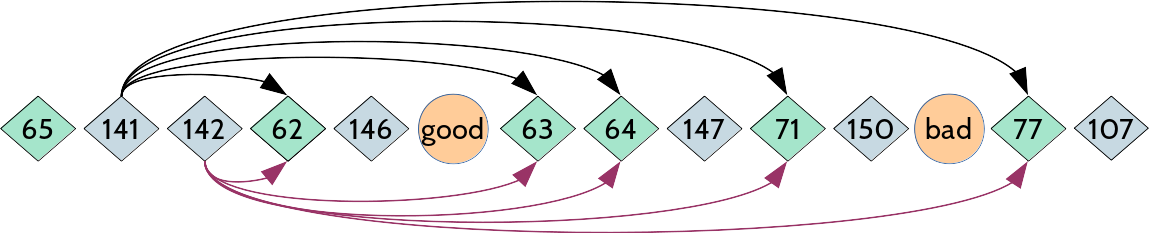
\includegraphics[scale=0.3]{img/solution-c}
\end{center}
\end{frame}

\begin{frame}{Ereignistypbasierte Regeln - Consumption Modes II}
\begin{center}
    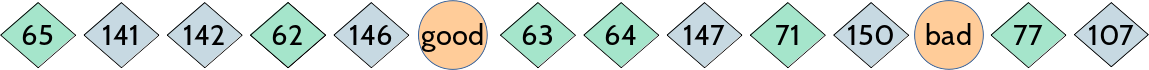
\includegraphics[scale=0.4]{img/stream-2}
\end{center}
\begin{exampleblock}{\textit{Continous Consumption Mode:}}
    \begin{center}
        \texttt{pattern[ \textcolor{red}{every} A $\rightarrow$ B]}\\\vspace{0.3cm}
        \texttt{select a,b from pattern[\textcolor{red}{every} a=StockTick(symbol='IBM') 
            $\rightarrow$ b=StockTick(symbol='SAP')];}
    \end{center}
    \begin{itemize}
        \item Jeder Initiator konsumiert nur nachfolgenden Detektor
    \end{itemize}
\end{exampleblock}

\begin{center}
    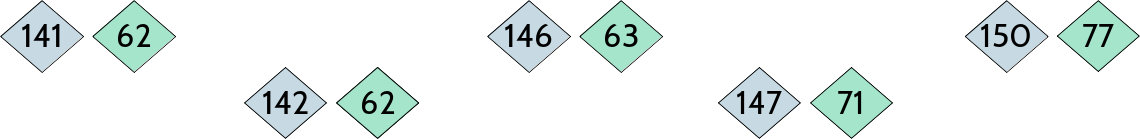
\includegraphics[scale=0.3]{img/solution-d}
\end{center}
\end{frame}


\begin{frame}{Ereignistypbasierte Regeln - Consumption Modes III}
\begin{center}
    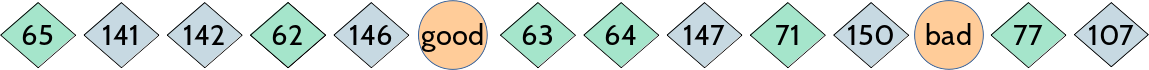
\includegraphics[scale=0.4]{img/stream-2}
\end{center}
\begin{exampleblock}{\textit{Continous \textcolor{red}{Detection} Mode:}}
    \begin{center}
        \texttt{pattern[  A $\rightarrow$ \textcolor{red}{every} B]}\\\vspace{0.3cm}
        \texttt{select a,b from pattern[ a=StockTick(symbol='IBM')
            $\rightarrow$\\ \textcolor{red}{every} b=StockTick(symbol='SAP')];}
    \end{center}
    \begin{itemize}
        \item Ein Initiator konsumiert alle nachfolgenden Detektoren
    \end{itemize}
\end{exampleblock}

\begin{center}
    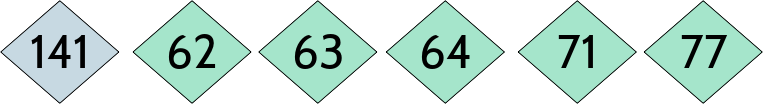
\includegraphics[scale=0.35]{img/solution-e}
\end{center}
\end{frame}

\begin{frame}{Ereignistypbasierte Regeln - Consumption Modes IV}
\begin{center}
    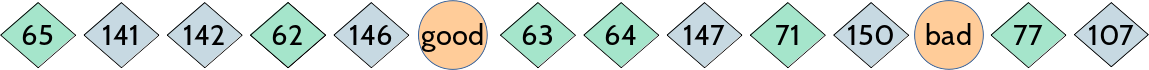
\includegraphics[scale=0.4]{img/stream-2}
\end{center}
\begin{exampleblock}{\textit{Regular Consumption Mode:}}
    \begin{center}
        \texttt{pattern[\textcolor{red}{every (}A $\rightarrow$  
        B\textcolor{red}{)}]}\\\vspace{0.3cm}
        \texttt{select a,b from pattern[\textcolor{red}{every (}%
        a=StockTick(symbol='IBM')$\rightarrow$  
        b=StockTick(symbol='SAP')\textcolor{red}{)}];}
    \end{center}
    \begin{itemize}
        \item Initiator sucht nach Detektor
        \item Initiatoren auf dem Pfad werden nicht betrachtet
    \end{itemize}
\end{exampleblock}

\begin{center}
    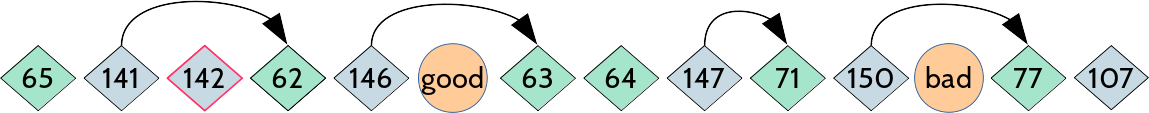
\includegraphics[scale=0.4]{img/solution-f}
\end{center}
\end{frame}

\begin{frame}{Ereignistypbasierte Regeln - Beispiel}
\begin{center}
    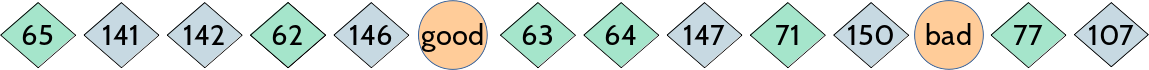
\includegraphics[scale=0.4]{img/stream-2}
\end{center}

\begin{block}{}
    \centering
    Wollen herausfinden, ob Nachrichtenmeldung Einfluss auf Aktienkurs hat
\end{block}

\begin{exampleblock}{}
    \begin{center}
    \texttt{select c from pattern[\textcolor{Magenta}{a=StockTick(symbol='IBM')} ->\\
    \textcolor{Bittersweet}{b=NewsTick(symbol='IBM' and message='bad')} ->\\
    \textcolor{blue}{c=StockTick(symbol='IBM' and price < 
    \textcolor{Magenta}{a}.price)}];} 
    \end{center}
 
\end{exampleblock}

\begin{center}
    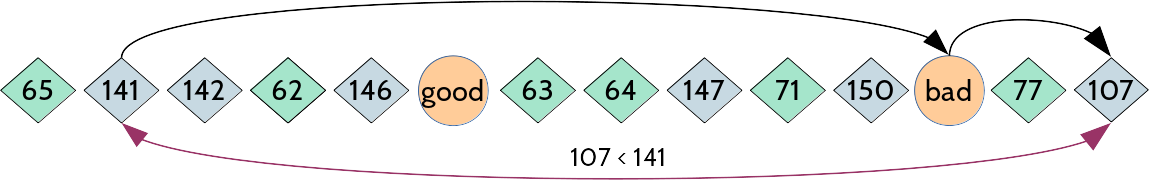
\includegraphics[scale=0.4]{img/solution-g}
\end{center}
\end{frame}

\begin{frame}{Komplexe Ereignisse}
\begin{center}
    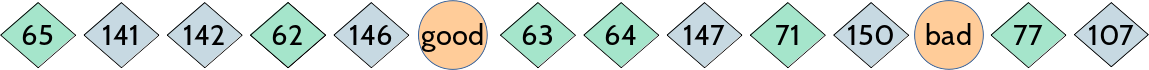
\includegraphics[scale=0.4]{img/stream-2}
\end{center}

\begin{block}{}
    \centering
    Wollen neues Ereignis: Mittelwert der letzten 6 Aktien einer Firma
\end{block}

\begin{exampleblock}{}
    \texttt{\textcolor{red}{insert into TargetEvent(symbol, average)}\\
        select symbol, avg(price)\\
        from StockTick\#groupwin(symbol)\#length\_batch(6);}\\\vspace{0.3cm}
    \texttt{select  * from \textcolor{red}{TargetEvent};}
\end{exampleblock}

\begin{center}
    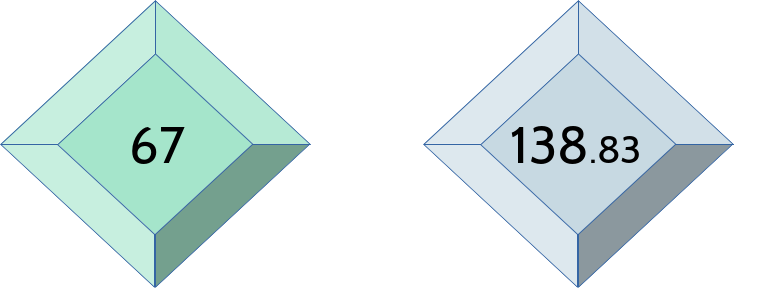
\includegraphics[scale=0.35]{img/solution-h}
\end{center}

\end{frame}

%%%%%%%%%%%%%%%%%%%%% MATCH_RECOGNIZE %%%%%%%%%%%%%%%
\begin{frame}{SQL: \texttt{Match\_Recognize}}
\begin{center}
    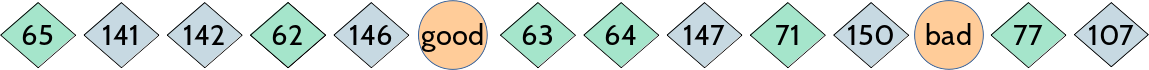
\includegraphics[scale=0.4]{img/stream-2}
\end{center}

\begin{exampleblock}{}
\texttt{select * from StockTick \textcolor{Bittersweet}{match\_recognize} (\\
\textcolor{Bittersweet}{partition} by symbol\\
\textcolor{Bittersweet}{measures} A[0].price as a0,A[1].price as a1, A[2].price as a2, 
B.price as b\\
\textcolor{Bittersweet}{pattern} \textcolor{red}{(A\{2,3\} B)}\\
\textcolor{Bittersweet}{define}\\
A as A.price < 150,
B as B.price >= 150)
}
\end{exampleblock}

\begin{center}
    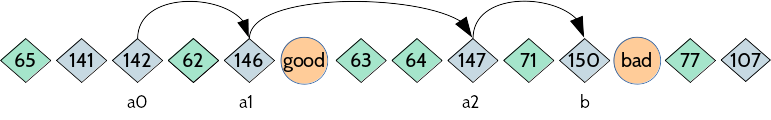
\includegraphics[scale=0.6]{img/solution-i}
\end{center}

\end{frame}

\begin{frame}{Fazit}
   \begin{itemize}
       \item Hohe Einstiegshürde
       \begin{itemize}
           \item EPL gut Dokumentiert
           \item Software eher nicht
       \end{itemize}
       \item Sehr großer Leistungsumfang
       \begin{itemize}
           \item Doku $>$ 900 Seiten
           \item TIMTOWDI
       \end{itemize}
       \item EPL-Prüfung mittels 
       EPL-Online\footnote{\url{https://esper-epl-tryout.appspot.com/epltryout/mainform.html}}
       \item Sehr leistungsfähige Architektur
   \end{itemize}
\end{frame}


%%%%%%%%%%%%%%%%%%%%%%%%%%%%%%%%%%%%%%%%%%%%%%%%%%%%%
\part{Endfolie}
\setbeamercolor{background canvas}{bg=green!3}
\begin{frame}

\framebreak
\begin{center}
\Large \textcolor{red!60}{{Danke für die Aufmerksamkeit.}}\\
\vspace{0.5 cm}
\end{center}
\begin{center}

\texttt{\scriptsize martin.steinbach@uni-rostock.de}\\

\end{center}



\end{frame}



\end{document}
